In the current section we present our framework for scalable and NUMA-aware producer-consumer data exchange. 
Our system follows the principle of separating mechanism and policy.
To this end, we consider two independent logical entities: 
\begin{enumerate}
	\item \emph{A single consumer pool (SCPool)} mechanism manages the tasks arriving to a given consumer while introducing the possibility of stealing some tasks by other consumers.
	\item A management policy is responsible for operating SCPools: the policy routes producers' requests to the appropriate consumers and initiates stealing between the pools. This way, the policy controls the system's behavior according to considerations of load-distribution, throughput, fairness, locality, etc.
	We are especially interested in a management policy suitable for Non-Uniform Memory Access (NUMA) architectures (see Figure~\ref{fig:system-fig}), where each CPU has its own memory, and accessing the memory of other CPUs is executed over an interconnect. As a high rate of remote memory accesses can decrease the overall performance, it is highly desirable for an SCPool of a consumer to reside at the RAM close to its own CPU. 
\end{enumerate} 

\paragraph{SCPool abstraction.}
\begin{algo}[!ht]
\caption{API for a Single Consumer Pool with stealing support.} 
\label{alg:scpool-api}
\begin{distribalgo}[1]
\scriptsize

\INDENT {\bf SCPool API:}
	\STATE produce(Task) \elcomment {Insert the task to the pool, returns false if no space left in the pool.}
	\STATE produceForce(Task) \elcomment {Inserts the task to the pool, expanding the pool if necessary. }
	\STATE consume() \elcomment {Retrieves a task from the pool, returns $\bot$ if no tasks in the pool are detected.}
	%\STATE getStealingScore() \elcomment {Returns a score corresponding to the amount of tasks to steal.}
	\STATE steal(SCPool from) \elcomment{Tries to steal a number of tasks from the given pool and move them to the current pool. Returns one of the stolen tasks or $\bot$. }%We guarantee that if there are tasks in the \emph{from} pool at the beginning of steal invocation, then either steal function returns a task, or there is another thread that returns a task during the steal execution.}
\ENDINDENT

\end{distribalgo}
\end{algo}

The SCPool API provides the abstraction of a single-consumer task pool with stealing support, see Algorithm~\ref{alg:scpool-api}.
A producer can invoke two types of insertion operations: \emph{produce}, which attempts to insert a task to the given pool and fails if the pool is full, and \emph{produceForce}, which always succeeds by expanding the pool on demand.
There are also two ways to retrieve a task from the pool: the owner of the pool (only) can call the \emph{consume} function; while any other thread can invoke the \emph{steal} function, which tries to transfer a number of tasks between the pools and return one of the stolen tasks. 
The pool must guarantee the following \emph{stealing property}, which is necessary for system liveness:
\begin{property}
If an SCPool is not empty at the beginning of a steal operation, then either the steal operation retrieves a task, or another thread retrieves a task during the steal execution.
\end{property}

A straightforward way to implement the API described above is to use a dynamic-size multi-producer multi-consumer FIFO queue (e.g., Michael-Scott queue~\cite{Michael:1996:SFP:248052.248106}).
In this case, both produce() and produceForce() enqueue a new task, while both consume() and steal() dequeue a task. In the next section we present SALSA, a much more efficient SCPool.

\begin{figure}[htb]
	\centering
	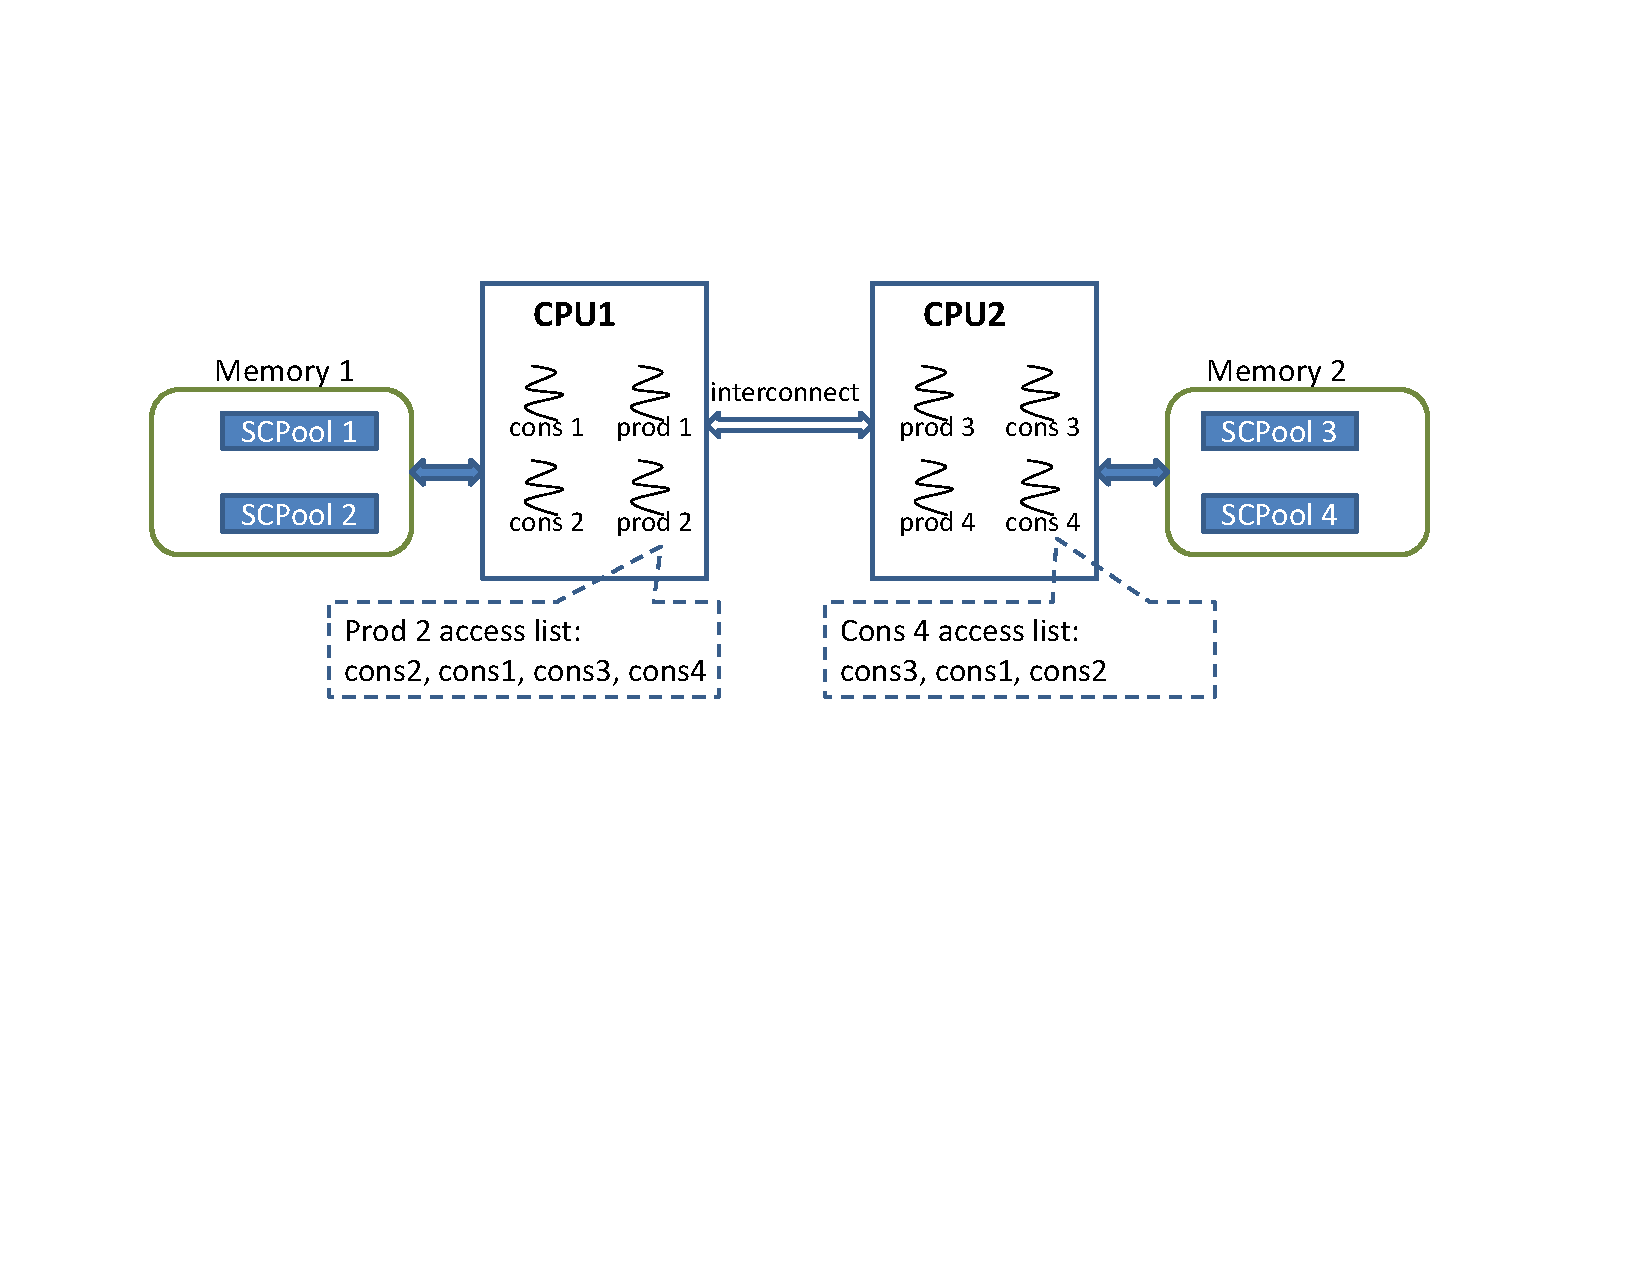
\includegraphics[width=0.7\textwidth]{figures/system-fig}
	\caption{\footnotesize{System overview of the management framework. In the given example the system is composed of two processors that are connected to their own memory banks (NUMA architecture). There are two producers and two consumers running on each processor, the data of each consumer is allocated at the closest available physical memory. A producer $p_i$ has an access list of consumers for task insertion. A consumer $c_i$ has an access list of consumers for task stealing. }}
	\label{fig:system-fig}
\end{figure}

\paragraph {Management policy.}
A management policy is generally defined by the way in which: (1) a producer chooses one of the SCPools to insert a task to, and when it chooses to use produce force; and (2) a consumer decides when to retrieve a task from its own pool and steal tasks from other pools. 
Note that the policy is independent of the underlying SCPool implementation. We believe that it is a subject for engineering optimizations, based on specific workloads and demands.


In the current work, we present a policy that exploits the locality properties of NUMA architectures and is aimed at achieving maximal throughput. If the individual SCPools themselves are lock-free and starvation-free, then our policy preserves these properties at the system level. Our policy is as follows:
\begin{itemize}
	\item {\bf Access lists.} Each process in the system (producer or consumer) is provided with an \emph{access list}, an ordered list of consumers, sorted according to their distance from that process (see Figure~\ref{fig:system-fig}). Intuitively, our policy is to have a producer mostly interact with the closest consumer, while stealing mainly happens inside the same processor node. 
	\item {\bf Producer's policy.} A producer inserting a task first calls the \emph{produce} function of the first SCPool in its access list. Note that a produce operation might fail if the pool is full, (which can be seen as evidence of that the corresponding consumer is overloaded).  In this case, the producer tries to insert the task into other pools, in the order defined by its access list. If all insertions fail, the producer invokes the \emph{produceForce} operation on the closest SCPool, which always succeeds (expanding the pool if needed). 
	\item {\bf Consumer's policy.} A consumer consumes tasks from its own SCPool. If its SCPool is empty, the consumer tries to steal tasks from other pools in the order defined by its access list. 
\end{itemize}



% The inter-pool communication policy is a subject to engineering optimizations and its optimal behavior should probably
% depend on the workload. For the purpose of our evaluation we propose the following approach. 
	% Producer policy. Each producer is provided with the list of all available consumers sorted according to the locality considerations of the given architectures. For example, in case of 
% In order to insert a task a producer first invokes a produce() operation on the closest consumer. If this operation fails, 
% then the closest consumer's pool is full (which could be evidence of an over-load of the given consumer thread) and the producer should 
% try to insert a task to another consumer. If neither consumer ... a producer finally invokes produceForce(), which expands the pool if necessary and always succeeds to insert the task. 
	% Consumer policy. A consumer works in a loop of consuming its own tasks. If the own pool of a consumer is empty, the consumer iterates over all other consumers and tries to steal tasks from there. 


